\documentclass[titlepage]{article}

\usepackage{authblk}
\usepackage{blindtext}
\usepackage{graphicx}

\title{Exercise 10 in Digital Tools for Finance}

\usepackage[backend=biber,style=bwl-FU,url=false,doi=false,eprint=false]{biblatex}
\addbibresource{bib.bib}

\author{Benjamin Clays\thanks{This is a thanks to someone who helped} and Seonbin Kim\thanks{another thank you note} and Max Kiefeer\thanks{this person also says thanks} and finally Valentyn Khmarskyi \thanks{a final thank you}}

\affil{Faculty of Business, Economics and Informatics, UZH}

\date{\today}

\begin{document}

\maketitle

\begin{abstract}
The abstract goes here, it's rather short and the text is not as wide as other text.

\end{abstract}

\section{Introduction}
\subsection{The intro of the introduction}
\blindtext[1]
\subsection{The body of the introduction}
\blindtext[5]
\subsection{The outro of the introduction}
\blindtext[2]

\section{This section introduces a table and a figure}
\subsection{Here is a table}

\begin{table}[h]
  \centering
    \begin{tabular}{| l c c r |}
    \hline
    $\alpha$ & 1 & 2 & 3 \\
    $\beta$ & 4 & 5 & 6 \\
    $\gamma$ & 7 & 8 & 9 \\
    $\delta$ & $\epsilon$ & $\zeta$ & $\eta$\\
    \hline
    \end{tabular}
  \caption{A simple table \protect\footnotemark[1]}
\end{table}

\subsection{The following subsection contains a figure}

\begin{figure}[h]
  \centering
    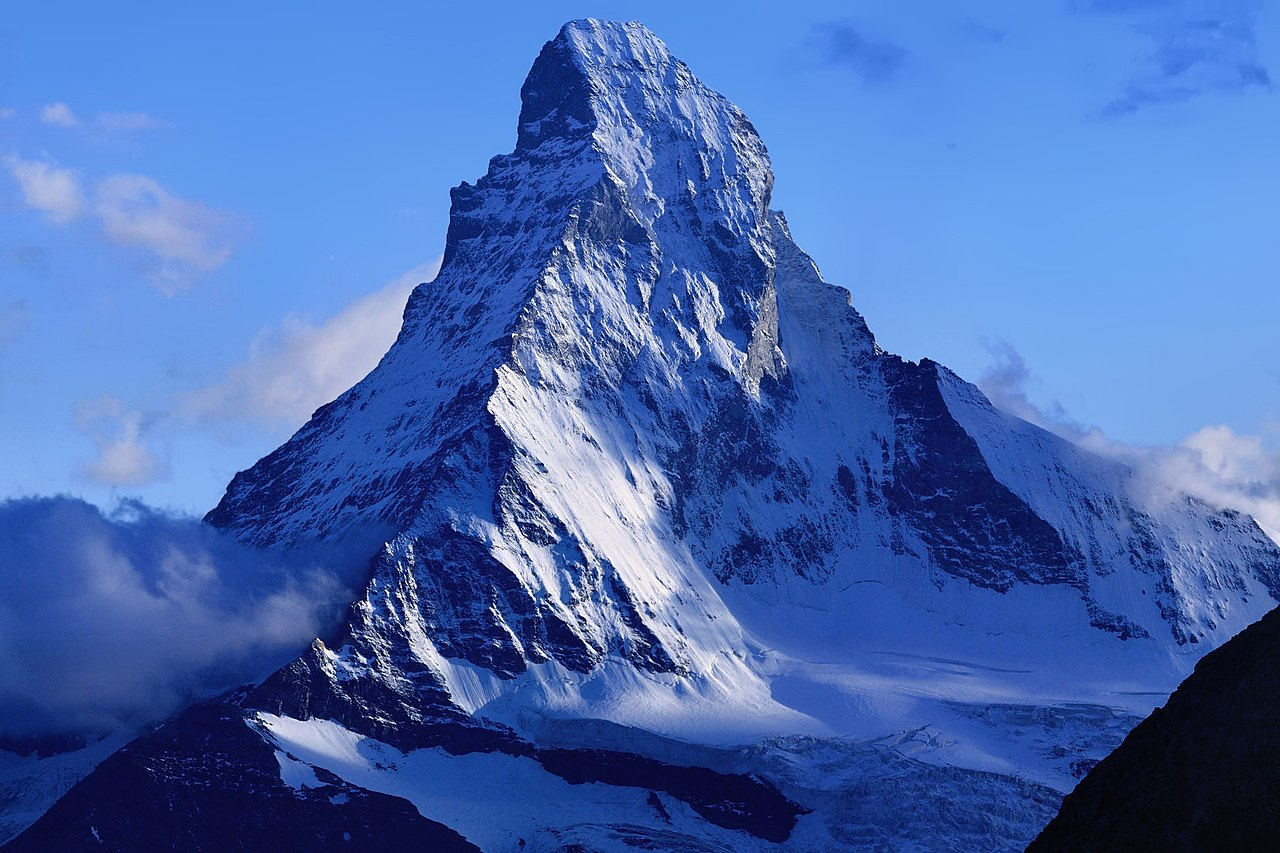
\includegraphics[width=0.5\textwidth]{matterhorn.jpg}
    \caption{A picture of Matterhorn.\protect\footnotemark[2]}
\end{figure}

\footnotetext[1]{This is a footnote for the table}
\footnotetext[2]{this is a footnote for the Matterhorn picture, to say that the picture is open-source, taken from the Wikipedia page of Matterhorn.
}

\section{Conclusion}
Here some text to cite a working paper: \cite{Kozlowski2020}. I can also cite \cite{Gormsen2020}, a finished paper. This concludes this article for the class of Digital Tools for Finance. I hope you enjoyed reading.
\newpage
\printbibliography

\end{document}